\documentclass[fr]{../../../eplsummary}
\usepackage[french]{varioref} % \vref and \vpageref
\usepackage{graphicx} % images
\usepackage{float} % images
\usepackage{url}
	\urlstyle{sf}
\usepackage[backgroundcolor=yellow]{todonotes} %% todonotes: \listoftodos & \todo{Some note or other.} & \missingfigure{}

% draw
\usepackage{tikz}
\usetikzlibrary{arrows,automata,calc}
\tikzset{
    %Define standard arrow
    >=stealth',
    % Define arrow style
    pil/.style={
           ->,
           thick,
           shorten <=2pt,
           shorten >=2pt,}
}
% \usepackage{qtree}    % dessiner des arbres %% => texlive-humanities

\definecolor{codeBlue}{rgb}{0,0,1}
\definecolor{webred}{rgb}{0.5,0,0}
\definecolor{codeGreen}{rgb}{0,0.5,0}
\definecolor{codeGrey}{rgb}{0.6,0.6,0.6}
\definecolor{webdarkblue}{rgb}{0,0,0.4}
\definecolor{webgreen}{rgb}{0,0.3,0}
\definecolor{webblue}{rgb}{0,0,0.8}
\definecolor{orange}{rgb}{0.7,0.1,0.1}

\usepackage{caption}
\renewcommand{\familydefault}{\sfdefault}

\usepackage{listings}		% Pour l'insersion de fichiers de codes sources.
\lstdefinelanguage{diff}{
  morecomment=[f][\color{blue}]{@@},     % group identifier
  morecomment=[f][\color{red}]-,         % deleted lines 
  morecomment=[f][\color{green}]+,       % added lines
  morecomment=[f][\color{magenta}]{---}, % Diff header lines (must appear after +,-)
  morecomment=[f][\color{magenta}]{+++},
}
\lstdefinelanguage{scala}{
  morekeywords={abstract,case,catch,class,def,%
    do,else,extends,false,final,finally,%
    for,if,implicit,import,match,mixin,%
    new,null,object,override,package,%
    private,protected,requires,return,sealed,%
    super,this,throw,trait,true,try,%
    type,val,var,while,with,yield},
  otherkeywords={=>,<-,<\%,<:,>:,\#,@},
  sensitive=true,
  morecomment=[l]{//},
  morecomment=[n]{/*}{*/},
  morestring=[b]",
  morestring=[b]',
  morestring=[b]"""
}
\lstset{
	  language=scala,
	  frame=single,
	  flexiblecolumns=true,
	  numbers=none, % left
	  stepnumber=1,
	  numberstyle=\ttfamily\tiny,
	  keywordstyle=\ttfamily\textcolor{blue},
	  stringstyle=\ttfamily\textcolor{red},
	  commentstyle=\ttfamily\textcolor{green},
	  breaklines=true,
	  extendedchars=true,
	  basicstyle=\ttfamily\scriptsize,
	  showstringspaces=false
	}

\IfFileExists{fourier.sty}{\usepackage{fourier}}{\typeout{! WARNING: Fourier package not included: skip it}}

\hypertitle{Languages and Translators}{8}{INGI}{2132}
{Matthieu Baerts\and Benoît Baufays\and Julien Colmonts\and Alex Vermeylen\and Hélène Verhaeghe}
{Pierre Schauss}

\listoftodos

%TODO merge
% \section{Chapter 1}
%
% \subsection{Compilation}
%
% \subsubsection{Compilers}
%
% A compiler is a program that \textbf{translates} a source program written in
% a \textbf{high-level} programming language such as Java, C\# or C, into an
% equivalent target program in a \textbf{lower level} language such as machine
% code, which can be executed directly by a computer.
%
% \begin{figure}[h]
%     \centering
%     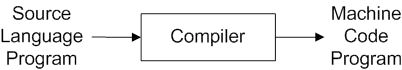
\includegraphics[width=8cm]{img/compilers.png}
%     \caption{Compilation}
% \end{figure}
%
% \paragraph{Input $\to$ output} 
% \begin{itemize}
%     \item Mapping names to memory addresses, stack frame offsets and
%         registers
%     \item Generate linear sequence of machine code instructions
%     \item Detecting any errors that can be detected
% \end{itemize}
%
%
% \subsubsection{Interpreters}
% Interpreter executed directly th high-level language program.
%
% \begin{figure}[h]
%     \centering
%     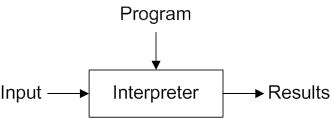
\includegraphics[width=8cm]{img/interpreters.png}
%     \caption{Interpretation}
% \end{figure}
%
% \begin{enumerate}
%     \item \textbf{Performance} : better with compilers (because
%         interpreter must parse and analyse the statement ot decode its
%         meaning \textit{every time} it execute that statement)
%     \item \textbf{Secrecy} : more difficult to understand program with
%         machine code
%     \item[but] sometime, the overhead of interpretation doesn't always
%         justify writing (or buying) a compiler. Like UNIX shell.
% \end{enumerate}
%
%
%
% \subsubsection{Programming languages}
%
% Specified in three steps :
% \begin{enumerate}
%     \item \textbf{Tokens} : like work in natural language
%     \item \textbf{Syntax}
%     \item \textbf{Semantics}
%     \item[Note] : The two first are described with formal notation, and
%         the last is described with natural language.
% \end{enumerate}
%
% \subsubsection{Machines Languages}
%
% A machine language program consists of a sequence of instructions and
% operands, usually organized so that each instruction and each operand
% occupies one or more bytes and so is easily accessed and interpreted.
%
% A machine instruction set and its behavior is often referred to as its
% \textbf{architecture}.
%
% \paragraph{Note:} Java Virtual Machine (JVM) is said \textit{virtual}
% because it is not necessarily implemented in hardware, rather it is
% implemente as a software.
%
% \subsection{Why study compilers}
%
% \begin{enumerate}
%
% \item Compilers are larger programs than the ones you’ve written
% in your programming courses. It is good to work with a program that is
% like the size of the programs you will be working on when you graduate.
%
% \item Compilers make use of all those things you have learned about
% earlier: arrays, lists, queues, stacks, trees, graphs, maps, regular
% expressions and finite state automata, context-free grammars and
% parsers, recursion and patterns. It is fun to use all of these in a real
% program.
%
% \item You learn about the language you are compiling (in our case, Java).
%
% \item You learn a lot about the target machine (in our case, both the
% Java Virtual Machine and the MIPS computer).
%
% \item Compilers are still being written for new languages and targeted
% to new computer architectures. Yes, there are still compiler-writing
% jobs out there.
%
% \item Compilers are finding their way into all sorts of applications
% including games, phones and entertainment devices.
%
% \item XML. Programs that process XML use compiler technology.
%
% \item There is a mix of theory and practice, and each is relevant to the
% other.
%
% \item The organization of a compiler is such that it can be written in
% stages, and each stage makes use of earlier stages. So, compiler writing
% is a case study in software engineering.
%
% \item Compilers are programs. And writing programs is fun.
% \end{enumerate}
%
%
%
%
% \subsection{Compiler work}
% \begin{figure}[h]
%     \centering
%     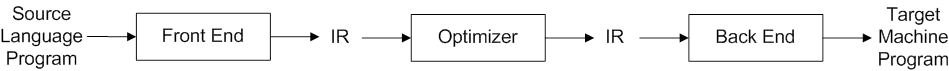
\includegraphics[width=8cm]{img/compilers_work.png}
%     \caption{Compiler work}
% \end{figure}
%
% \subsubsection{Front end}
% \begin{itemize}
%     \item[-] Analyse the input program to determining its meaning
%     \item[-] Source language dependent (target language independent)
% \end{itemize}
%
% \begin{figure}[h]
%     \centering
%     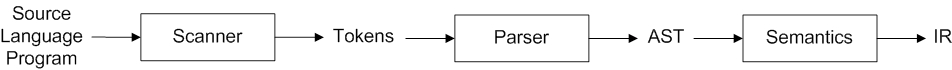
\includegraphics[width=8cm]{img/frontend.png}
%     \caption{Front end : analysis}
% \end{figure}
%
% \begin{itemize}
%     \item \textbf{Scanner} : With a input stream of character make a
%         stream of tokens identifiers, literal, reserved word, operatos
%         and separators
%     \item \textbf{Parser} : Produce an abstract syntax tree (AST)
%     \item \textbf{Semantics} : Declaring name in a symbol table, ,
%     looking up names as they are referenced for determining their types,
%     assigning types to expressions, and checking the validity of types.
% \end{itemize}
%
% \subsubsection{Back end}
% \begin{itemize}
%     \item[-] Produces a target machine program having the same meanig and is source 
%     \item[-] Source language dependent (target language independent)
% \end{itemize}
%
% \begin{figure}[h]
%     \centering
%     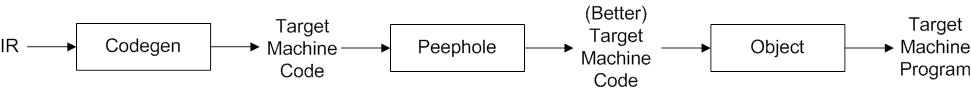
\includegraphics[width=8cm]{img/backend.png}
%     \caption{Back end : analysis}
% \end{figure}
%
% \begin{itemize}
%     \item \textbf{Codegen} : choosing what target machine instructions
%         to generate. (information collected in earlier phases)
%     \item \textbf{Peephole} : Generated instruction locallu for wasteful
%         instructions sequences such as branches to branches and
%         unnecessary load/stroe pairs.
%     \item \textbf{Object} : Constructs a single machine code executable
%         program
% \end{itemize}
%
% \subsubsection{Middle end}

\chapter{Lexique}
\todo{ben}

CFG : Context-Free Grammar

PEG : Parsing Expression Grammar : grammaire non-ambigue qui est exprimmée comme une CFG mais pour éviter les ambiguités, on prend tjs la première dérivation qui marche.




\chapter{Synthèse du livre}
\section{Chapitre 1 : Compilation} % LN, Matth
\subsection{Compiler}
\paragraph{Compilateur} Programme qui traduit un programme source écrit dans un langage haut-niveau en un programme équivalent écrit en langage de bas niveau (code machine le plus souvent).\\
Ces deux programmes ont des comportements identiques.

\subsubsection{Programming language}
\paragraph{Langage de programmation} Un langage artificiel dans lequel un programmeur écrit un programme pour contrôler le comportement d'une machine.\\
On définit un language de programmation par 3 étapes:
\begin{itemize}
	\item les tokens: "mot-clé" du langage
    \item la syntaxe et la construction du langage: comment écrire un programme qui fonctionne
    \item la sémentique du langage: sens des phrases.
\end{itemize}

\subsubsection{Machine language}
\paragraph{Langage machine} (ou ensemble d'instructions) Un langage facilement interpreté par l'ordinateur lui-même. Chacune des instruction ou des opérations un ou plus de bytes et est facilement acédé et interprété. On parle également d'architecture pour l'ensemble d'instructions et le comportement d'une machine.\\
On distringue plusieurs niveaux de complexités (CISC: \textit{Complex Instruction Set Computer} ou 

: \textit{Reduced Instructive Set Computer}). Il faut plusieurs instructions RISC pour obtenir une instruction CISC.\\
Comme les registres sont très rapides, un ordinateur va essayer de garder au maximum les données dans les registres.

\paragraph{Machine virtuelle} L'architecture est implémentée en software. Les étapes de l'analyse du compilateur pour produire le programme de sortie sont:
\begin{itemize}
	\item Mapper les noms aux adresses mémoires, frames de la pile et registres.
    \item Générer la liste linéaire des instructions machines.
    \item détecter les erreurs
\end{itemize}
Dans le cas d'un interpréteur, le code high-level est exécuté directement.\\
Avantages d'un compilateur (par rapport à un interpréteur) :
\begin{itemize}
	\item Performances: du code machine est plus rapidement exécuter, l'interpréteur doit lui redécoder à chaque fois les lignes de codes pour les transformer en instructions.
    \item Secret: le code source est très difficile à déduire depuis un code machine.
\end{itemize}
Avantages d'un interpréteur :
\begin{itemize}
	\item Pas un problème pour les scripts (petits programmes très peu appelés).
    \item Contrôle: le code source est disponible, facilement modifiable (pour des scripts).
    \item Langage machine dépend de la machine alors qu'avec un interpréteur, il est portable.
\end{itemize}

\subsection{Why should we study compilers?}
\begin{itemize}
	\item Ce sont de très grands programmes (comme ceux que nous étudirons plus tard)
    \item Il fait usage de tout ce que nous avons vu avant
    \item Cela permet d'apprendre sur le langage
    \item on en apprend sur la machine visée
    \item Il existte encore du boulot de compilation pour les nouveaux langages
    \item Ils se retrouvent partout
    \item Les programmes utilisent du XML se servent de technologies de compilation
    \item Mix de théorie et pratique
    \item Comme un compilateur peut être écrit en étapes, c'est un cas d'étude d'ingénérie logicielle
    \item écrire des programmes est chouette
\end{itemize}

\subsection{How does a compiler work? Phases of compilation}
On peut diviser en plusieurs étapes.

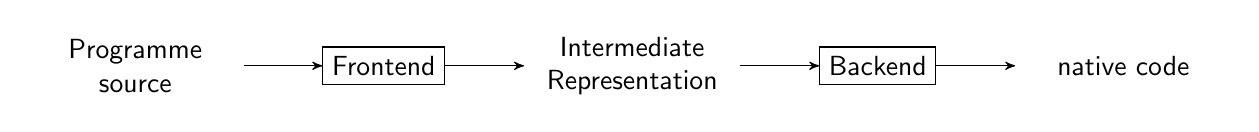
\begin{tikzpicture}
	\node[text width=2.5cm,align=center] (A) {Programme source};
    \node[draw, shape=rectangle] (B) [right=of A] {Frontend};
	\node[text width=2.5cm,align=center] (C)[right=of B] {Intermediate Representation};
    \node[draw, shape=rectangle] (D) [right=of C] {Backend};
	\node[text width=2.5cm,align=center] (E) [right=of D] {native code};
	\path[->] (A) edge (B)
              (B) edge (C)
              (C) edge (D)
              (D) edge (E);
\end{tikzpicture}

\subsubsection{Frontend}
\begin{itemize}
	\item Analyse du programme pour en deviner le sens
    \item dépend uniquement du langage de départ
    \item peut être décomposé:
\end{itemize}
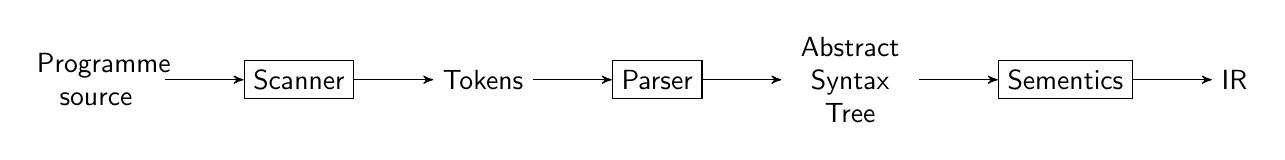
\begin{tikzpicture}
	\node[text width=1.5cm,align=center] (A) {Programme source};
    \node[draw, shape=rectangle] (B) [right=of A] {Scanner};
	\node (C)[right=of B] {Tokens};
    \node[draw, shape=rectangle] (D) [right=of C] {Parser};
	\node[text width=1.5cm,align=center] (E) [right=of D] {Abstract Syntax Tree};
    \node[draw, shape=rectangle] (F) [right=of E] {Sementics};
	\node (G) [right=of F] {IR};
	\path[->] (A) edge (B)
              (B) edge (C)
              (C) edge (D)
              (D) edge (E)
              (E) edge (F)
              (F) edge (G);
\end{tikzpicture}

\subsubsection{Backend}
\begin{itemize}
	\item Prend le IR et produit le code machine
    \item Dépend de la machine d'arrivée uniquement
    \item peut-être décomposé en phases
\end{itemize}
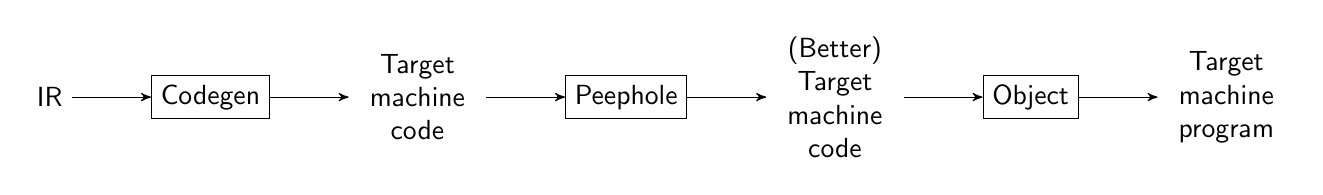
\begin{tikzpicture}
	\node (A) {IR};
    \node[draw, shape=rectangle] (B) [right=of A] {Codegen};
	\node[text width=1.5cm,align=center] (C)[right=of B] {Target machine code};
    \node[draw, shape=rectangle] (D) [right=of C] {Peephole};
	\node[text width=1.5cm,align=center] (E) [right=of D] {(Better) Target machine code};
    \node[draw, shape=rectangle] (F) [right=of E] {Object};
	\node[text width=1.5cm,align=center] (G) [right=of F] {Target machine program};
	\path[->] (A) edge (B)
              (B) edge (C)
              (C) edge (D)
              (D) edge (E)
              (E) edge (F)
              (F) edge (G);
\end{tikzpicture}
Avec:
\begin{itemize}
	\item Codegen: Choisi les instructions adéquates
    \item Peephole: Cherche à faire un peu d'optimisation locale du code
    \item Object: liste les différents modules et construit un programme exécutable
\end{itemize}

\subsubsection{Middle end}
Il peut y avoir l'ajout d'un optimisateur entre le grontend et le backend. Celui-ci à pour but d'améliorer le code intermédiare:
\begin{itemize}
	\item Il organise le programme en blocks
    \item Recherche la durée de vie des variables (next-use information)
    \item Élimine des sous-expressions et des \textit{constaints folding} ($x+4=9$ si on sait que $x=5$), regarde à l'allocation des registres
    \item Met les invariants hors des boucles, remplace les multiplication par des additions (car moins couteuse)
\end{itemize}

\subsubsection{Avantage de la décomposition}
\begin{itemize}
	\item Réduit la complexité
    \item Permet un dévelopement en parallèle
    \item Permet une réutilisation (un seul backend pour tous les langages pour une même machine
\end{itemize}

\subsubsection{Compiling to a Virtual Machine: New Boundaries}
Les programmes Java sont d'abord compilés en un fichier \texttt{.class} éxécutable sur la machine virtuelle. La machine virtuelle, quant à elle, est un interpréteur qui observe le code qu'on lui donne et compile les parties critiques (hotspot) qui sont les plus souvent appelées. Il fait aussi du \textit{in-lining}, c'est-à-dire remplacer des appels de méthode par leur code.\\
On peut considérer le \texttt{.class} comme dans un IR (Intermediate Representation) et JavaC comme le frontend. La machine virtuelle est du coup le backend.\\
Sur Windaube, ils ont implémenté une machine CLR (Commun Langage Runtime). Suivant une technique appelée JIT (Just In Time), le CLR compile chaque méthode en code natif et utilise ce code lorsque la méthode est appelée.

\subsubsection{Compiling JVM code sur une architecture en registre}
La stratégie consistant à fournir du code intermédiare pour une machine virtuelle a plusieurs avantages :
\begin{itemize}
	\item Le code intermédiare est compact
    \item De gros efforts ont eété fait pour optimiser ces machines virtuelles pour qu'elles s'exécute très rapidement (ex: Java, LOL)
    \item Le fait de ne compiler que les régions spéciales permettent d'aller plus vite que de compiler l'entièreté du code.
\end{itemize}

\subsection{An overview of the j-\-- to SVM compilers}
j-\-- est un sous-ensemble de Java: non-trivial, orienté objet, supporte les classes, méthodes, champs, messages, statements, expressions et types primitifs. Son compilateur est écrit en Java d'une manière orienté objet.

\subsubsection{j-\-- compiler organization}
Le début est la \texttt{main}. Après avoir lu les arguments, elle crée le parser et le scanner. Ensuite:
\begin{itemize}
	\item \texttt{compilationUnit()} au parser pour obtenir l'AST.
    \item \texttt{preAnalyze()} au n\oe ud principal de l''arbre pour déclarer les types et classes dans la table des symboles.
    \item \texttt{analyze()} pour déclarer les noms et chercher les types
    \item \texttt{codegen()} pour gérer le code
    \item S'il y a des erreurs, on cherche s'il y en a d'autres et on arrête après.
\end{itemize}

\subsubsection{Scanner}
Le scanner scanne les tokens à la demande et les classes suivant que ce soit des identifiants (\texttt{main, myMethod}), des tokens réservés (\texttt{import, public, class}) ou des littéraux (tout le reste sans les séparateurs: \texttt{"Hello World", 3}, etc.).

\subsubsection{Parser}
Le parser est spécifique à la syntaxe du langage et est effectué en \textit{recursive descent}.

\subsubsection{AST}
L'abstract syntax tree est une représentation sous forme d'arbre pour le programme source. Il permet de rendre explicite la structure syntaxique. Chacune des classes des nœuds étendent une même classe et implémente 3 méthodes: \texttt{preAnalyze()} (déclarer les types), \texttt{analyze()} (déclarer les variables localesà et \texttt{codegen()} (pour générer le code).

\subsubsection{Types}
Un type indique comment se comporte quelque chose. Java est dit statiquement typé car les types sont déterminés à la compilation.\\
Dans le compilateur j-\--, on crée une classe type pour placer les différents types.

\subsubsection{\texttt{preAnalyze()} and \texttt{analyze()}}
\texttt{preAnalyze()} est le premier à vérifier le type. Il recherche les symboles au dessus du AST (déclare les types importés et ceux déclarés par les class).\\
\texttt{analyze()} reprend là où \texttt{preAnalyze()} s'est arrêté. Il s'occupe de:
\begin{itemize}
	\item Type checking: trouver le type de chaque expression
    \item Accessibilité: Regarde aux \texttt{public}, \texttt{protected} et \texttt{private}
    \item Member finding: vérifie les signatures.
    \item Tree rewriting: réécrit certains tree
\end{itemize}

\subsubsection{Stack Frames}
L'analise s'occupe aussi de calculer l'offset des variables locales dans la stack frame (block continu de mémoire au-dessus de la pile \textit{run-time}). On peut ainsi savoir l'espace repris par une méthode à chacune de ses invocations.

\subsubsection{\texttt{codegen()}}
Permet de générer le byte code pour la JVM. Un outil (\texttt{CLEmitter} existe et permet de construire la table des constantes et de générer les références utilisées par la JVM pour les noms et constantes. Permet de calculer des offsets de \textit{brckets} et les adresses. Calcule les coûts (espace mémoire) des variables et l'espace de calcul nécessaire dans une méthode. Et pour finir, il construit le fichier \texttt{.class}.

\subsubsection{j-\-- compiler source tree}
Pour ajouter une opération, on doit modifier le scanner pour reconnaitre les nouveaux tokens, modifier le parser pour reconnaitre l'expression, implémenter l'analyse sémentique et finalement la génération du code allant avec cette opération.




\section{Chapitre 2 : Lexical Analysis} % LN, Matth
\subsection{Introduction}
La 1\iere{} étape est le cassage en tokens.
\paragraph{Lexical tokens}: éléments composant les programmes. Ils sont décrits par la syntaxe lexicale du langage.
\paragraph{Lexical analysis}: procédé permettant d'identifier les lexical tokens dans le programme. On peut séparer les tokens lexicaux en catégories: les mots réservés, les identifiants, les \textit{strings literal}, les opérateurs et les séparateurs.

\subsection{Scanning tokens}
\paragraph{Scanner} Un scanner peut être défini comme un programme écrit par le programmeur du compilateur ou bien générée automatiquement par une liste de regex. Les espaces peuvent séparer des tokens mais pas tout le temps. Un scanner peut être décrit par des machines à états finis.
\paragraph{State transition diagram} diagramme dans lequel les nœuds représentent les états, les flèches dirigées représentes des mouvement d'un état à l'autre suivant ce qui est scanné. Si un caractère scanné n'est sur aucune flèche, on choisi celle non étiquetée.\\

C'est facile d'implémenter une machine à état fini en terme de code, il suffit de mettre les choix comme des \texttt{if} (ou \texttt{switch}) et les cycles comme des \texttt{while}.\\
Pour reconnaître les mots réservés, on pourrait faire une machine à états mais elle serait trop complexe. On préfère lister les mots réservés dans une table et faire un \textit{lookup} à chaque fois qu'on reconnait un identifiant. Pour les opérateur, on utilise une machine à états finis qui agit comme un grand switch entre les différents opérateurs possibles. Concernant les espaces, on les ignore simplement, tout comme les commentaires.

\subsection{Regular Expressions (regex)}
On dit que les regex définissent un langage de strings sur un alphabet. Les regex peuvent prendre les formes suivantes:
\begin{itemize}
	\item Si $a$ est dans l'alphabet, alors le regex a décrit le langage consistant en les strings $a$. On appelle ce langage $L(a)$
    \item Si $r$ et $s$ sont des regex, alors leur concaténation $rs$ est aussi une regex décrivant le langage de tous les strings possibles obtenus par concaténation d'un string du langage $r$ et d'un string de langage $s$. On appelle ce langage $L(rs)$
    \item Si $r$ et $s$ sont des regex, $L(r|s)$ décrit le langage composé des strings de l'un ou l'autre langage
    \item Si $r$ est un regex, $L(r*)$ décrit le langage formé par concaténation de zéro ou plusieurs instances de $r$ ($\epsilon$ représente la string vide)
    \item $\epsilon$ est le langage contenant uniquement la string vide
    \item $r$ et $(r)$ sont les mémes regex. Les parenthèses sont utilisées pour grouper les regex.
\end{itemize}

\subsection{Finite State Automate (FSA)}
Pour tout langage décrit par une regex, il existe un diagramme à transition d'état.
\paragraph{Automate à états finis} (Finite State Automate) c'est $F = (\Sigma, S, s_0, M, F)$ où:
\begin{itemize}
	\item $\Sigma$ est l'alphabet
    \item $S$ est l'ensemble des états
    \item $s_0 \in S$ est l'état initial
    \item $M$ est l'ensemble de mouvements possibles d'un état à un autre ; $m(r, a) = S$ où $r, s \in S$ et $a \in \Sigma$
    \item $F \in S$ est l'ensemble des états finaux
\end{itemize}
On dit qu'un automate fini reconnait un langage. Une phrase sur l'alphabet appartient au langage si en partant du start, on arrive sur un état final après avoir suivit les changement d'états correspondant à la phrase. Il existe un moyen automatique de générer un FSA à partir de regex.

\subsection{Non-Deterministic Finite State Automate (NFA) vs. Deterministic FSA (DFA)}
\paragraph{DFA} automate à états finis où il n'y a pas de $\epsilon$-move et où un seul chemin peut -être pris suivant un même input.
\paragraph{NFA} automate à états finis qui permet plusieurs chemins pour le même input ainsi que des mouvements.

\subsection{Regular expressions to NFA}
On utilise les constructions de Thompson:
\begin{itemize}
	\item $a$:\\
    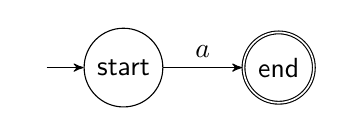
\begin{tikzpicture}
		\node[state] (A) [initial, initial text={}] {start};
    	\node[state] (B) [right=of A, accepting] {end};
		\path[->] (A) edge node[above] {$a$} (B); % [bend left]
	\end{tikzpicture}
	\item $rs$:\\
    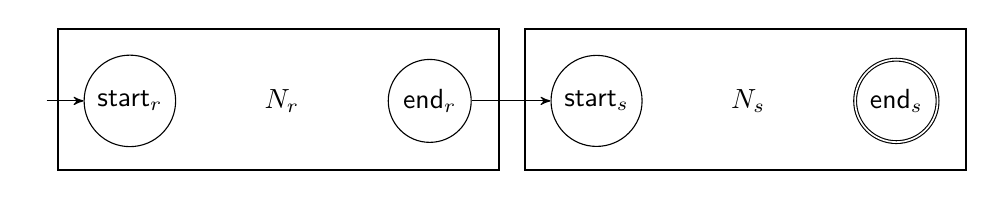
\begin{tikzpicture}
		\node[state] (A) [initial, initial text={}] {start$_r$};
    	\node        (B) [right=of A] {$N_r$};
    	\node[state] (C) [right=of B] {end$_r$};
		\node[state] (D) [right=of C] {start$_s$};
    	\node        (E) [right=of D] {$N_s$};
    	\node[state] (F) [right=of E, accepting] {end$_s$};
		\path[->] (C) edge (D);
        \draw[thick] ($(A.north west)+(-0.5,0.5)$) rectangle ($(C.south east)+(0.5,-0.5)$);
        \draw[thick] ($(D.north west)+(-0.5,0.5)$) rectangle ($(F.south east)+(0.5,-0.5)$);
	\end{tikzpicture}
	\item $r|s$:\\
    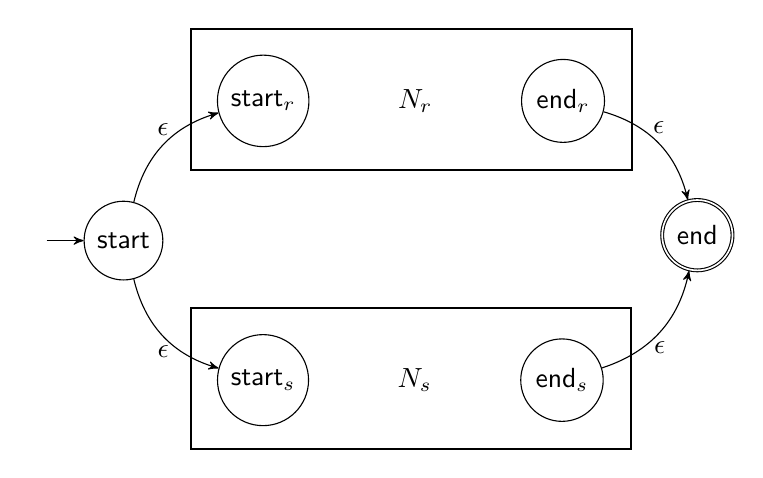
\begin{tikzpicture}
    	\node[state] (0) [initial, initial text={}] {start};
		\node[state] (A) [above right=of 0]{start$_r$};
    	\node        (B) [right=of A] {$N_r$};
    	\node[state] (C) [right=of B] {end$_r$};
		\node[state] (D) [below right=of 0] {start$_s$};
    	\node        (E) [right=of D] {$N_s$};
    	\node[state] (F) [right=of E] {end$_s$};
    	\node[state] (G) [below right=of C, accepting]{end};
		\path[->] (0) edge[bend left] node[above] {$\epsilon$} (A);
		\path[->] (0) edge[bend right] node[below] {$\epsilon$} (D);
		\path[->] (C) edge[bend left] node[above] {$\epsilon$} (G);
		\path[->] (F) edge[bend right] node[below] {$\epsilon$} (G);
        \draw[thick] ($(A.north west)+(-0.5,0.5)$) rectangle ($(C.south east)+(0.5,-0.5)$);
        \draw[thick] ($(D.north west)+(-0.5,0.5)$) rectangle ($(F.south east)+(0.5,-0.5)$);
	\end{tikzpicture}
	\item $r*$:\\
    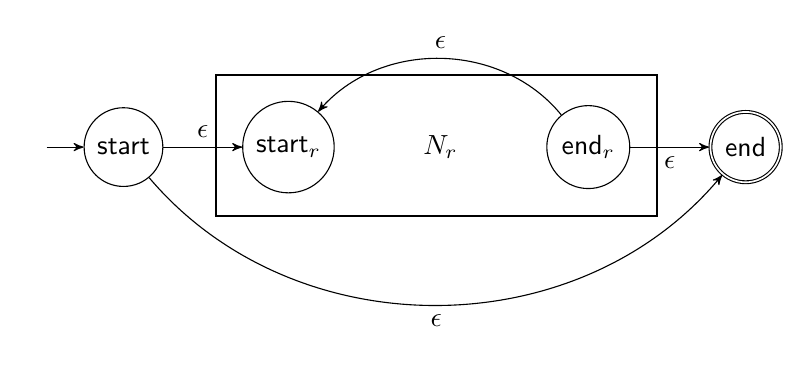
\begin{tikzpicture}
    	\node[state] (0) [initial, initial text={}] {start};
		\node[state] (A) [right=of 0]{start$_r$};
    	\node        (B) [right=of A] {$N_r$};
    	\node[state] (C) [right=of B] {end$_r$};
    	\node[state] (D) [right=of C, accepting]{end};
		\path[->] (0) edge node[above] {$\epsilon$} (A);
		\path[->] (0) edge[bend right=50] node[below] {$\epsilon$} (D);
		\path[->] (C) edge[bend right=50] node[above] {$\epsilon$} (A);
		\path[->] (C) edge node[below] {$\epsilon$} (D);
        \draw[thick] ($(A.north west)+(-0.5,0.5)$) rectangle ($(C.south east)+(0.5,-0.5)$);
	\end{tikzpicture}
	\item $\epsilon$:\\
    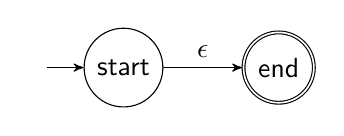
\begin{tikzpicture}
		\node[state] (A) [initial, initial text={}] {start};
    	\node[state] (B) [right=of A, accepting] {end};
		\path[->] (A) edge node[above] {$\epsilon$} (B);
	\end{tikzpicture}
\end{itemize}

\subsection{NFA to DFA}
Pour toutes NFA, il existe une DFA équivalente. On arrive à la trouver grâce aux $\epsilon$-closure.
\paragraph{$\epsilon$-closure($s$)} c'est un ensemble incluant $s$ ainsi que tous les états atteignables à partir de $s$ grâce uniquement à des $\epsilon$-moves.
\paragraph{$\epsilon$-closure($S$)} c'est un ensemble incluant $S$ ainsi que tous les états atteignables à partir de chaque élément $s$ de $S$ grâce uniquement à des $\epsilon$-moves.


\subsection{Minimal DFA}
On cherche à combiner les états les plus probables. On va recréer des états grâce à des partitions. Les partitions initialles sont \textit{final} et \textit{non-final}. On doit s'assurer que pour chacun des états, le mouvement d'un symbole particulié reflète celui dans l'ancien DFA. Pour une partition particulière, chaque symbole d'input doit induire un mouvement vers la même partition.

\subsection{JavaCC: Tool for generating scanner}
JavaCC est un outil pour générer une analyse lexicale à partir de regex ainsi qu'un parseur à partir d'une grammaire hors contexte.\\
Lorsque l'on scanne un token, on considère tous les regex correspondant à l'état actuel et on choisi celui qui contient le plus de caractères.\\
Il existe 4 types de regex:
\begin{itemize}
	\item SKIP: regex jeté
    \item MORE: on continue après
    \item TOKEN: crée un token et est retourné au parseur
    \item SPECIAL-TOKEN: crée un token spécial ne participant pas au parsing
\end{itemize}

\section{Chapitre 3 : Parsing}
\subsection{Introduction}
\paragraph{Parsing} action de mettre les tokens ensemble pour créer des entités syntaxiques plus grandes (expressions, instructions, méthodes, définition de class, ...).

La première fonction du parser est d'assumer la validité syntaxique du programme. Il doit être capable d'identifier une erreur et la reporter (erreur et le numéro de ligne). Il doit également être capable de ne pas s'arrêter après une erreur ete de chercher les autres (pour ne pas reporter qu'une seule erreur à la fois). La deuxième fonction du parseur est de fournir une représentation du programme parsé. On choisit souvent une représentation en arbre car ce type de représentation est facile à analyser et à "décorer" d'informations.

\subsection{Context-Free Grammars and Languages}
\subsubsection{Backus-Naur Form (BNF) and its extensions}
On définit les langages de programmation de manière récursive pour la plupart.
\begin{itemize}
	\item[$::=$] : "\textit{peut être écrit comme}", sigle de la définition
    \item[$|$] : "ou"
    \item[$[X\rfloor$] : $X$ est optionnel % bug latex: si on met \item[[x]] (il pense que le 1er ']' ferme l'option de l'item.
    \item[$\{X\}$] : \textit{Keene closure}, $X$ apparait de 0 à plusieurs fois.
\end{itemize}

\subsubsection{Grammar and the Language it describes}
\paragraph{Context-Free grammar} Une grammaire sans contexte est un tuple $G=(N,T,S,P)$ où:
\begin{itemize}
	\item[$N$] est un ensemble de symboles non terminaux
    \item[$T$] est un ensemble de symboles terminaux
    \item[$S \in N$] est un non terminal appelé symbole de départ
    \item[$P$] est un ensemble de règles de production
\end{itemize}

\paragraph{Derivation} Séquence d'applications de règles de production, démarrant du symbole de départ pour arriver à l'expression voulue («~$\Rightarrow$~» est le symbole de la relation de dérivation).

\paragraph{Directly derive} Lorsqu'un string de symboles dérive d'un autre en une seule étape.

\paragraph{Language $L(G)$} On dit que le langage $L(G)$, décrit par une grammaire $G$, consiste en tous les strings ne comprenant que des symboles terminaux pouvant être dérivés du symbole de départ.

\paragraph{Left-most derivation} Dérivation dans laquelle, à chaque étape, le string suivant est dérivé en applicant une règle de production réécrivant un non terminal le plus à gauche.

\paragraph{Right-most derivation} Dérivation dans laquelle, à chaque étape, le string suivant est dérivé en applicant une règle de production réécrivant un non terminal le plus à droite.

\paragraph{Sentential form} Chaque string de terminaux ou non terminaux qui peut être dérivé à partir d'un symbole de départ.

\paragraph{Parse tree} Arbre illustrant les dérivations effectuées depuis un symbole de départ (racine) pour arriver à une expression (feuilles).

\subsubsection{Ambiguous Grammars and unambiguous grammars}

\paragraph{Ambiguous sentence} Une phrase par laquelle il existe plusieurs dérivations possibles. (2 arbres pour représenter $id + id * id$

\paragraph{Ambiguous grammar} Une grammaire qui décrit au-moins une phrase ambigüe.

\paragraph{Unambiguous grammar} Une grammaire ne décrivant que des phrases à dérivation unique (qu'elle soit \textit{left} ou \textit{right}). Il y a néenmoins des ambiguités qui subsistent:
\begin{lstlisting}
S ::= if (E) S
   | if (E) S else S
   | s
E ::= e
if (e) if (e) s else s
\end{lstlisting}
Deux représentations:\\

\begin{tabular}{ll}
{\begin{lstlisting}[frame=leftline]
if (e)
    if (e)
        s
    else
        s
\end{lstlisting}}\hspace{1cm}
&
{\begin{lstlisting}[frame=leftline]
if (e)
    if (e)
        s
else
    s
\end{lstlisting}}
\end{tabular}
\vspace{.5cm}

Pour résoudre cette ambiguité, on groupe le \texttt{else} avec le \texttt{if} précédent.\\
Il y a aussi ambiguité avec $x.y.z$: est-ce un \textit{field selection}, un nom de package, un nom de class, etc. Pour résoudre cela, un nœud \textit{Ambiguous Name} est placé dans l'AST et est revurevu par le compileur après la déclation des types (\textit{type declaration}).\\

Pour les parseur des langages décrits par une grammaire \textit{context-free}, on utilise une \textit{pushdown} stack avec \textit{backtracking}. Lorsque le \textit{backtracking} n'est pas nécessaire, on parle de parsing déterministe. Deux types de parsing déterministes:
\begin{itemize}
	\item Top-Down: on part du symbole de départ pour arriver à la fin.
    \item Bottom-up: on part de la phrase et on remonte jusqu'au symbole de départ.
\end{itemize}

\subsection{Top-Down Deterministing Parsing}
Deux types de top-down: recursive descent ou $LL(1)$. Tous deux vont de gauche à droite, regarde et scanne un seul symbole à la fois. Le parseur démarre du symbole initial comme goal initial. Il va scanner la phrase d'input et parser les entités syntaxique représentées par le symbole de départ.

\subsubsection{Parsing by recursive descent}
On doit avoir une méthode par parser, chaque non terminal suivant la règle de production adaptée. Suivant le prochain symbole non scanné, la méthode décide de la règle à appliquer et scanne les terminaux utiles et les non-terminaux en utilisant les méthodes par les parsers. Ces méthodes construisent également les nœuds AST. Le scanner a quelques méthodes utiles pour aider à décider de la règle de production adéquate :
\begin{itemize}
	\item \texttt{have(TOKEN)}: renvoie \texttt{true} si le token est présent.
	\item \texttt{mustBe(TOKEN)}: renvoie \texttt{true} si le token est présent ou une erreur sinon.
	\item \texttt{see(TOKEN)}: regarde si le token est présent sans le scanner.
\end{itemize}
Pour certaines grammaires, il faut regarder plus loin que le token suivant pour savoir ce qui est présent en premier et pour savoir quelle loi de dérivation utiliser. On a un \textit{Lookahead} scanner définit qui permet de voir plus loin qu'un symbole. Pour récupérer des erreurs, les \texttt{mustBe}, lorsqu'il rencontre un token inatendu, scanne jusqu'à trouver celui qu'il veut jusqu'à se ree remettre dans un état à nouveau correct.

\subsubsection{$LL(1)$ parsing}
Contrairement au recursive descent, ici, la stack est explicite. Le 1\ier $L$ veut dire \textit{left-to-right scan}, le 2\ieme pour \textit{left-most derivative} et le $1$ pour le fait qu'on regarde un seul symbole à la fois.\\
Au tout début, on place le symbole temrinal initial sur la pile. Suivant le token scanné, on remplace le symbole sur la pile par celui qui correspond suivant la table de parsing. Lorsqu'un terminal est trouvé sur la pile et si c'est bien celui qui est scanné, il est retiré de la pile et un nouveau token est scanné.\\

Chaque grammaire a une table de parsing unique. Pour créer la table, si $\alpha$ et $\beta$ sont des strings (pouvant être vides) de terminaux et non terminaux, $table[Y,a]=i$ où $i$ est le numéro de la règle, $Y ::= X_1, X_2,..., X_n$ si soit $X_1, X_2,..., X_n \Rightarrow a\alpha$ ou $X_1, X_2,..., X_n \xrightarrow{*} \epsilon$ et il y a une dérivation $S$\# $ \Rightarrow \alpha Y a \beta$.\\
Pour arriver à établir cette table, on fait usage de deux algorithmes: \texttt{first} et \texttt{follow}.\\

Calcul de $first(X)$ pour tous les $X$ dans la grammaire:
\begin{itemize}
	\item For each terminal $x$, $first(x) = \{x\}$.
	\item For each non-terminal $X$, $first(X) = \{\}$.
	\item If there is a rule $X ::= \epsilon$ in $P$, add $\epsilon$ to $first(X)$.
	\item Repeat until no new symbols are added to any set: For each rule$ Y ::= X_1 X_2 ... X_n \in P$, add all symbols from $first(X_1 X_2 ... X_n)$ to $first(Y)$.\\
\end{itemize}

Calcul de $first(X_1 X_2 ... X_n)$:
\begin{lstlisting}[mathescape]
Set S = first(X$_1$).
i = 2
While $\epsilon$ $\in$ S and i $\le$ n {
    S = S - $\epsilon$
    Add first(X$_i$) to S
    i = i+1
return S
\end{lstlisting}

$Follow(X)$:
\begin{itemize}
	\item $follow(S) = \{$\#$\}$.
	\item $follow(X) = \{\}$ for all non-terminals X $\ne$ S.
	\item Repeat until no new symbols are added to any set:\\
	\hspace*{1em} for each rule $Y ::= X_1 X_2... X_n \in P$,\\
    \hspace*{2em} for each non-terminal $X_i$,\\
	\hspace*{3em} add $first(X_{i+1} X_{i+2}... X_n) - {\epsilon}$ to $follow(X_i)$, and\\
	\hspace*{4em} if $X_i$ is the rightmost symbol or $first(X_{i+1} X_{i+2}... X_n)$ contains $\epsilon$,\\
    \hspace*{4em} add $follow(Y)$ to $follow(X_i)$.\\
\end{itemize}

Construire une table de parsing $LL(1)$ pour une grammaire $G=(N,T,S,P)$:\\
For each non-terminal $Y$ in $G$,\\
\hspace*{1em}For each rule $Y ::= X_1 X_2...X_n \in P$ with number $i$,\\
\hspace*{2em}For each terminal $a$ $\in$ $first(X_1 X_2... X_n) - \{\epsilon\}$, add $i$ to $table[Y, a]$.\\
\hspace*{2em}If $first(X_1 X_2... X_n)$ contains $\epsilon$, for each terminal (or \#) in $follow(Y)$, add $i$ to $table[Y, a]$.\\

Une grammaire est dite $LL(1)$ si la table de parsing produite n'a pas de conflits. Toute grammaire $LL(1)$ est non ambigue.\\
On peut avoir des grammaire non $LL(1)$ mais $LL(k)$ avec $k>1$ (on regarde alors $k$ symboles). On peut transformer certaines grammaires non $LL(1)$ en une équivalente $LL(1)$  dans certains cas:
\begin{align*}
	\text{left recursive: } X &::= X\alpha & X &::= \beta X'\\
    X &::= \beta & \Rightarrow X' &::= \alpha X'\\
    & & X' &::= \epsilon\\
    \text{left factoring: } X &::= \alpha \beta & X &::= \alpha X'\\
    X &::= \alpha \gamma & \Rightarrow X' &::= \beta\\
    & & X' &::= \gamma     
\end{align*}

\subsection{Bottom-up deterministic parsing}
On passe!!

\subsection{Parser Generation using Java CC}
On utilise une structure syntaxique EBNF (\textit{extended BNF}. On peut définir ainsi des parseurs $LL(k)$ récursive descent. Le fichier \texttt{j--.jj} contient donc les regex pour la structure lexicale ainsi que les règles syntaxiques du langage.\\
Entre \texttt{PARSER\_BEGIN(JavaCCParser)} et \texttt{PARSER\_END(JavaCCParser)} sont définies des fonctions utiles et utilisées dans le parser généré. On définit premièrement le symbole de départ (\texttt{compilationUnit}) en fonction de non-terminaux de niveaux inférieurs.\\
La syntaxe EBNF est:
\begin{itemize}
	\item $[a]$: 0 ou 1
    \item $(a)^*$: 0 ou plusieurs
	\item $a|b$: $a$ ou $b$
    \item $()$: grouping
\end{itemize}
La déclaration de non terminaux ressemble à une méthode java. Il y a un type de retour, un nom, peut avoir des arguments et à un corps de méthode. Il y a un bloc précédent celui-là dans lequel les variables locales sont déclarées.\\
Lorsqu'il est nécessaire de regarder plusieurs symboles après l'actuel, on utilise la méthode \texttt{LOOKAHEAD(<token>)}. Il y a deux méthodes pour récupérer des erreurs : \textit{shallow} et \textit{deep} (utilisé par j-\--). Dans le corps d'un non terminal, on catch les erreurs du parseur. On choisit alors à quel token on veut reprendre (\textit{skip to token}). Il y a donc premièrement affichage d'une erreur puis récupération par shipping. Les avantages d'un parser autogénéré (JavaCC) sont:
\begin{itemize}
	\item Structure lexicale mieux expliquée
    \item Construction EBNF possible
    \item Lookahead possible et facile
    \item Conflit de choix reporté
    \item Mécanisme de récupération d'erreur sophistiqué utilisable.
\end{itemize}


\subsection{Bactracking parsing (not in the book)} %LN

Avec le backtracking parsing, on peut parser n'importe quel langage décrit par une CFG. On va dériver en left most à partir du symbol initial en choisisant la première règle de dérivation. Tant que les terminaux déjà obtenu match le string qu'on veut matcher alors on continue, sinon on revient à l'étape pérédente et on choisit la règle de dérivation suivante.

Exemple:

Suivant la grammaire :
\begin{lstlisting}
S ::= ASA
S ::= ASB
S ::= A
A ::= a
B ::= b
\end{lstlisting}

Si on souhaite parser $aab$, on a les étapes suivantes :
\begin{lstlisting}
S
S => ASA
S => ASA => aSA
S => ASA => aSA => aASAA
S => ASA => aSA => aASAA => aaSAA
S => ASA => aSA => aASAA => aaSAA => aaASAAA
S => ASA => aSA => aASAA => aaSAA => aaASAAA => aaaSAAA
!! backtrack !!
S => ASA => aSA => aASAA => aaSAA => aaASAAA
!! backtrack a nouveau car pas d autre regle pour A !!
S => ASA => aSA => aASAA => aaSAA
S => ASA => aSA => aASAA => aaSAA => aaASBAA
S => ASA => aSA => aASAA => aaSAA => aaASBAA => aaaSBAA
!! backtrack !!
S => ASA => aSA => aASAA => aaSAA => aaASBAA
!! backtrack a nouveau car pas d autre regle pour A !!
S => ASA => aSA => aASAA => aaSAA
S => ASA => aSA => aASAA => aaSAA => aaAAA
S => ASA => aSA => aASAA => aaSAA => aaAAA => aaaAA
!! backtrack !!
S => ASA => aSA => aASAA => aaSAA => aaAAA
!! backtrack a nouveau car pas d autre regle pour A !!
S => ASA => aSA => aASAA => aaSAA
!! backtrack a nouveau car pas d autre regle pour S !!
S => ASA => aSA => aASAA
!! backtrack a nouveau car pas d autre regle pour A !!
S => ASA => aSA
S => ASA => aSA => aASBA
S => ASA => aSA => aASBA => aaSBA
... (on a compris l idee)
\end{lstlisting}

\subsection{Packrat parsing (not in the book)} %LN

Pour éviter le coût du backtrack parsing (qui peut être exponentiel si à chaque fois on se retrouve à devoir prendre la dernière dérivation), on utilise de la mémorization. On obtient donc un algorithme en O(input*\#production).

On va pour chaque index dans l'input essayer de parser via toutes les règles possibles et stocker le résultat ainsi que l'index de fin de l'expression. On peut ainsi aller de l'index le plus grand au plus petit en utilisant les résultats précedemment calculés.





\section{Chapitre 4 : Type checking}

\subsection{Introduction}

Du \textit{type checking}, c'est faire de l'analyse sémantique. On y applique les opérations suivantes :
\begin{itemize}
	\item Détermine le type de tous les noms et expressions
    \item type checking: on vérifie les types des opérations
    \item analyse du stockage pour savoir la place reprise par les variables locales
    \item réécriture de l'arbre AST pour rendre explicite certaines constructions.
\end{itemize}

\subsection{j-\-- types}
\subsubsection{Introduction}
On a soit des types primitifs (\texttt{int, boolean, char}), soit des types référentiels (\texttt{array}, type définit par une déclaration de classe, \texttt{java.lang.Object}, etc.).

\subsubsection{Type representative and class objects}
On défini deux objets \textit{placeholder} pour prendre la place des types non résolu encore :
\begin{itemize}
	\item Type Name: est résolu en faisant un lookup dans le contexte (représentation dy symbol table)
    \item Array Type Name: on résoud le type des éléments de l'array et on l'encapsule dans une \textit{Class Object} utilisé ensuite dans l'array.
\end{itemize}
On utilise cette technique car le type défini ce qu'il nous faut et on peut utiliser des types temporaire avant la résolution.

\subsection{j-\-- Symbol Table}
\subsubsection{Contexts And Idefns: Declaring and Looking Up Types and Local Variables}
La table des symboles est représentée par un arbre d'objets contexts, chacun correspondant à une région de scope du programme et contenant un mapping des noms vers ce qu'ils sont. Dans chacun des contextes asociés aux méthodes de classes, on associe un champ \textit{surrounding context} qui pointe vers le contexte englobant le bloc correspondant. Deux types de Idefns dans les entrées de la table:
\begin{itemize}
	\item Type Name defn qui encapsule juste un type
    \item Local variable defs qui défini une variable locale en encapsulant son nom, type et un offset dans la frame stack.
\end{itemize}

\subsubsection{Finding Method and Field Names in Type Objects}
\todo{LN}

\subsection{Pre-Analysus of j-\-- program}
\subsubsection{An introduction to pre-analysis}
L'analyse sémantique requiert 2 traversés de l'AST car des classes et méthodes peuvent être déclarées après une référence. La première analyse est un une \texttt{preAnalyze()} qui va:
\begin{itemize}
	\item déclarer les types importés (\texttt{JCompilationUnit} level)
    \item déclarer les class définies par l'user (\texttt{JClassDeclaration} level)
    \item déclarer des champs (\texttt{JFieldDeclaration} level)
    \item déclarer les méthodes (\texttt{JMethodDeclaration} et \texttt{JConstructorDeclaration} level)
\end{itemize}

\subsubsection{\texttt{JCompilationUnit.preAnalyse()}}
Rôle:
\begin{itemize}
	\item Créer le \texttt{CompilationUnitContext}
    \item Déclarer les types implicites \texttt{java.lang.String} et \texttt{java.lang.Object}
    \item Déclarer les types importés
    \item Déclarer les types définis par les déclarations de classe
    \item Invoquer \texttt{preAnalyze()} pour chacun des déclarations de type dans la Compilation Unit
\end{itemize}

\subsubsection{\texttt{JClassDeclaration.preAnalyse()}}
Rôle:
\begin{itemize}
	\item Crée le \textit{Class context}
	\item Résoud le type \texttt{super} de la classe
	\item Crée le \texttt{CLEmitter} associé
	\item Ajoute header, name et modifier du CLE
	\item Invoque \texttt{preAnalyze} sur les membres de la classe
	\item Rajoute un constructeur explicite s'il n'y a pas
	\item Produit le \textit{Class object}.
\end{itemize}

\subsubsection{\texttt{JMethodDeclaration.preAnalyse()}}
Rôle:
\begin{itemize}
	\item Résoud les types des paramètres et du \texttt{return}
	\item Vérifie si l'\textit{abstract modifier} est propre
	\item Calcule du descripteur de méthode (codification de la signature en string (\texttt{(I)I}: consomme un \texttt{int}, renvoie un \texttt{int} ; ([L\texttt{java.lang.String;})V : prend une liste ([) de strings (L\texttt{java.lang.String;}), revoie \texttt{void})
	\item Appelle \texttt{partialCodeGen()} pour générer le code de la méthode sans le corp pour que l'objet class ait au-moins les informations de l'interface des méthodes (paramètre et le type du \texttt{return}
\end{itemize}

\subsubsection{\texttt{JFieldDeclaration.preAnalyse()}}
Rôle:
\begin{itemize}
	\item Vérifie qu'un champs n'est pas déclaré \texttt{abstract}
	\item Résoud le type du champ
	\item Génère le code bytestream pour la JVM pour la déclaration des champs
\end{itemize}

\subsubsection{Symbol Table built by \texttt{preAnalyse()}}
L'étape de pré-analyse ne déclare aucune variable locale. On a donc un arbre partiel qui est construit.

\subsection{Analayse of j-\-- programs}
Lors de l'analyse, on va effectuer une discrete recursive:
\begin{itemize}
	\item Réécriture de champs et d'initialisation de variables locales comme des assignements de variables normales
    \item Déclaration des paramètre formet et des variables locales
    \item Allocation des ressources sur la stack frame
    \item Calcul des types des expressions
    \item Reclassification des noms ambigus
    \item Modification de l'arbre
\end{itemize}

\subsubsection{Top the AST}
\subsubsection{Declaring Formal parameters ad local variable}
\subsection{Visitor Pattern and the AST traversal Mechanism}

\section{Chapitre 5: JVM and Bytecode}
Voir slides...
\begin{itemize}
	\item \texttt{ifge, ifeq, ifnull, ifnonnull}, etc.: compare l'élément au top de la stack par rapport à 0
    \item \texttt{if\_icmeq, if\_icmgt}, etc.: compare les 2 éléments au top de la stack
\end{itemize}


\section{Chapitre : Garbage Collection} \todo{quel chapitre?} %LN


Une première manière de manager la mémoire est de manière explicit (malloc/free). Plusieurs désaventage: peut mener à bcp d'erreur (double free, seg fault,...), programmation modulaire bcp plus complexe (il faut se mettre d'accord sur qui free, qui malloc,...).

L'automatisation permet de donner l'illusion d'avoir une infinité de mémoire. Le programmeur ne doit également plus penser à cela. Cela retire également un tas de bugs.


\subsection{Reference Counting}

Chaque objet retient le nombre de réference vers lui-même, incrémentation/décrémentation à chaque création/destruction de référence. Lorsque le compte tombe à 0, suppression de l'objet.

Cette méthode est rapide, sûre et marche dans la plupart des cas (si il y a des références circulaire (A ref B et B ref A), ca ne marche pas).

\subsection{Mark \& Sweep}

Phase 1 : Mark : on démare de root, on trace l'object graph en marquant tout les objets atteints.

Phase 2 : Sweep : on itère sur tout les objets du heap, on supprime les objets non marqué et on clear les marks.

On peut le faire en Depht-first Search (avec ou sans récursion) ou alors en pointer reverse.

Le cout peut être très élevé si il y a peu à jetter. Si plus de 50\% de la heap est concervée, on augmente la taille de la heap.

L'allocation de donnée dans le heap se fait par :
Lorsqu'un objet demande un chunk, on peut donner n'importe quel block de taille >= celle demandée. C'est plus efficace de maintenir des listes des blocks disponible par taille.


Le mark and Sweep permet de gerer les cycles. Par contre, il peut y avoir des problème de fragmentation et un cout d'allocation grand.


\subsection{Copying collection : Cheney algorithm}

On splitte la heap en 2 : from-space et to-space.

Initialement tout les chunck utilisé sont dans le from-space. Au lieu de marquer les chuncks utilisés, on les place dans le to-space. Tout en maintenant à l'ancien emplacement une référence vers le nouvel emplacement.
On déplace ainsi petit-à-petit en suivant les liens. Lorsque l'algo est fini, on inverse les utilisations des deux espaces (from devient to et to deviens from).

Les aventages sont : facile d'allouer de la mémoire (à la fin), pas de fragmentation (compactage automatique), le temps est proportionnel au nombre d'objets vivants. Par contre, il faut le double d'espace mémoire.

\subsection{Generational collection}

On ne fait du tris que dans les objets concidéré comme "jeune", c'est à dire lorsqu'ils ont survécu à plusieurs passage du garbage collector. On a alors une siscion dans la mémoire entre jeune et vieux. Lorsqu'un objet devient vieux, il est déplacé dans la partie vieux.


\section{DSL \& Scala} % Alex

\subsection{Les constructeurs}

En scala, un constructeur "simple" n'a pas besoin d'être défini.

Exemple :

\begin{lstlisting}
class vehicle(name: String, price:Int) {

}

var car = new vehicle("Ferrari", 100000);
\end{lstlisting}

Il est également possible de définir un constructeur "custom" de cette façon là :

\begin{lstlisting}
class vehicle(name: String, price:Int) {

	def this(name: String) = {
		this(name, 10)
	}
}
\end{lstlisting}

\subsection{Les variables}

Deux mots-clefs permettent de définir des variables en Scala : \texttt{val} et \texttt{var}. La différence entre les deux est que les valeurs associées au "vars"
peuvent être modifiées alors que pour les "vals", une seule assignation est possible.

\begin{lstlisting}
var jizz = "jizz"
jizz = "baufays" //Autorise

val poulpe = "poulpy"
poulpe = "manteau louche" //INTERDIT !
\end{lstlisting}

A noter qu'il n'est pas n"cessaire d'écrire le type. Cependant, on peut le faire :

\begin{lstlisting}
val answer: Int = 42 
\end{lstlisting}

\subsection{pure OO}

En Scala, tout est un objet (pas de type primitif). Ainsi, chaque opération est un appel de méthode. de ce fait, "1 + 2" peut s'écrire "1.+(2)".

\subsection{Fonction anonymes}

\begin{lstlisting}
val plusOne = (x:Int) => x+1
plusOne(5) // va retourner 6
\end{lstlisting}

\subsection{closure}

\begin{lstlisting}
//	plusFoo	can reference any values/variables in scope	

var foo = 1
val plusFoo = (x:Int) => x+foo

plusFoo(5) //return 6

foo = 5
plusFoo(5) //now return 10
\end{lstlisting}

\subsection{Higher order function}

Deux choses importantes :

1. l'utilisation de \_ :

\begin{lstlisting}
val nums = List(1,2,3)

nums.exists(_ == 2) //return true
\end{lstlisting}

2. une fonction peut prendre une autre fonction en paramètre.

\subsection{classes}

\subsubsection{object}

Les \texttt{object} sont comme des classes statiques. Donc :

\begin{lstlisting}
object Test extends App
\end{lstlisting}

représente la déclaration d'une classe anonyme qui étend App ainsi que la création d'une unique instance "Test" de cette classe anonyme.\\
A noter que "App" est utilisé comme la classe main en Java.\\
A noter également que les méthodes définies à l'intérieur d'un object sont des méthodes statiques, au sens \#Java8 du terme.

\subsubsection{getters and setters}

Ils n'esistent pas en Scala. Il suffit de faire comme si on accédait a une champ en Java. "nomDeLaClasse.Champ = 'Hélène roule en tracteur'".

\subsubsection{companion object and apply}

Un objet compagnon est un objet qui porte le même nom que la classe qu'il accompagne.
La spécificité étant que la classe peut accéder au membres privés de l'objet et vice versa.

La méthode "apply" est une méthode qui agit un peu comme un constructeur pour les objects et qui peut être utilisée avec les classes comme sucre syntaxique :

\begin{lstlisting}
//Exemple 1

class Calculator(brand: String) {	
	def add(m: Int, n: Int): Int = m + n	
}

object Calculator {	
	def apply(brand: String) = new Calculator(brand)	
}

object Test extends App {	
	
val c1 = new Calculator("HP") //sucre syntaxique pour Calculator.apply("HP")
val c2 = Calculator("HP") // TODO : Different de celui du dessus ???
}


//Exemple 2

class Test(n: Int) {
	def apply(m: Int) = {
    	return m+n
    }
}

object Main extends App {
	val t = Test(1)
    println(t(2)) // va imprimer '3'
}
\end{lstlisting}

\subsubsection{operator overload}

Il suffit de réecrire une méthode avec le même nom...

\subsection{Mutability}

\todo{What is this fuk ? En quoi c'est cool/pas cool ? \#poulpe}

\subsection{Null and options}

Null, c'est nul ! Difficle à gérer. Si une variable peut être nulle, il faut checker, sinon risque de \texttt{NullPointerException}.

A la place, il faut utiliser le type \texttt{Option[T]}. Selon le cas, cela va nous renvoyer \texttt{Some(x)} si x existe, \texttt{None} dans l'autre cas.

\subsection{Currying (et safraning, paprikaning, etc.)}

On peut définir plus qu'une séquence d'arguments.

\begin{lstlisting}
def add(a)(b) = a+b
add(1)(2)
\end{lstlisting}

\subsection{Call by name}

En général, par exemple en \#Java8\footnote{pour les intimes...}, on fait du call by value. C'est à dire que les arguments d'une fonction seront toujours évalué avant l'exécution de la fonction. De ce fait, on connait la valeur de ces arguments. Par exemple, si un des argument est "2+2", on l'évaluera à "4"
avant de lancer l'exécution de la fonction.

Dans le call by name, on peut utiliser des fonctions comme argument, et celles-ci ne seront évaluées que lorsque l'on en aura besoin (un peu comme le "lazy" qu'on a vu en OZ).

L'avantage du by value est que la fonction utilisée en argument n'est évaluée qu'une seule foi. L'avantage du by name est que si on a pas besoin d'évaluer la fonction on ne le fera pas.

Les deux méthodes sont équivalentes dans le cas de fonctions pures et si les exécutions terminent. Par exemple :

\begin{lstlisting}
object Test {
   def main(args: Array[String]) {
        delayed(time());
   }

   def time() = {
      println("Getting time in nano seconds")
      System.nanoTime
   }
   def delayed( t: => Long ) = {
      println("In delayed method")
      println("Param: " + t) //1
      wait(5000)
      println("Param: " + t) //2
   }
}
\end{lstlisting}

Ici, si on fait du by value, les deux print imprimeront la même chose. Par contre, dans le cas du by name, la fonction sera recalculée et on aura deux valeur différente à imprimer. \todo{correct ?}\\

Notons qu'en Scala, l'utilisation du by value est celle pas défaut. Si on veut du by name, on doit ajouter "=>" devant le type de l'argument.

\subsection{implicit conversion}

Permet de convertir automatiquement un type en un autre pour pouvoir appliquer certaines opérations. Exemple :

\begin{lstlisting}
import ComplexImplicits._	
	
object ComplexImplicits {	
	implicit def Double2Complex(value : Double) = new Complex(value,0.0) 	
	}	

object MyComplex extends App {	
	
	val d = Complex(1)(2)	
	val e = 1+d	//Ici, le Int 1 va automatiquement etre converti en Complex
    			//via la methode Double2Complex
}
\end{lstlisting}

\subsection{implicit classes}

\todo{heu ... ?}

\subsection{implicit parameters}

En gros, c'est une loucherie qui permet de remplacer automatiquement un argument d'une fonction si on apelle la fonction sans cet argument. Après...

\todo{A completer}

\subsection{Traits}

Les traits sont à la frontière entre les interfaces et les classes abstraites.

En effet, le trait est plus riche que l'interface en ce sens qu'elle peut contenir une implémentation. En outre, le trait diffère de la classe abstraite par le fait que son constructeur ne peut contenir aucun paramètre et, il est lié dynamiquement, permettant un héritage multiple.

Ce n'est pas un objet (on ne peut pas l'instancier).
C'est un truc entre les interfaces et les classe abstraite. Comme une interface, c'est implémenté par une classe et cela contient un certain nombre de signatures de méthodes que la classe devra implémenter. Mais comme une classe abstraite, il y a un certain nombre de méthodes déjà implémentées. Par contre un trait ne peut pas être instancié.

Exemple :

\begin{lstlisting}
trait Comp {

def < (that : A): Boolean

def > (that : A): Boolean = {...}
def >= (that : A): Boolean = {...}
...

}
\end{lstlisting}

\subsection {Monads}
Il s'agit d'une structure e donnée qui défini à la fois \texttt{map} (prend un iterable et applique la fonction passée en argument) et \texttt{flatMap} (idem que map mais avec un flatten en plus: \texttt{[1, [2]]} $\Rightarrow$ \texttt{[1, 2]}: on aura plus qu'une seule liste à la fin) et \texttt{Unit}.\\

Tous les types \texttt{M[T]} donc en gros des listes de \texttt{T} (structure de données génériques) et qui ont deux opérations spéciales: \texttt{flatMap} et \texttt{unit}
\begin{itemize}
	\item[\texttt{flatMap}]: prend une fonction en argument et l'applique à tous les éléments de la structure et va faire un flatten (\texttt{[1, [2]]} $\Rightarrow$ \texttt{[1, 2]}: on aura plus qu'une seule liste à la fin)
    \item[\texttt{unit}]: va prendre une valeur en argument (du type générique de la structure) et va créer une structure avec cette élément dedans. Ex: \texttt{List(x)}: on aura une liste avec \texttt{x} comme premier élément de la structure.
\end{itemize}


\subsection{Yield}
Va faire une espère de link dans le type du premier du for:
\begin{lstlisting}
val A = Array(1,2)	
val B = List(1,2)
for (i <- A; j <- B) yield (i,j) 	
// Array((1,1),	(1,2), (2,1), (2,2))	
for (i <- B; j <- A) yield (i,j) 	
// List((1,1), (1,2), (2,1), (2,2))
\end{lstlisting}




\chapter{Questions d'exam}

\section{Lexical Anal. IS-IS}

\section{Grammar}

\subsection{Give an example of ambiguity in a real programming language. How is it managed in practice?}
\todo{explain}
\begin{align}
E ::=& E+E & & E ::= TE'\\
E ::=& E\times E & & E' ::=  +TE'\\
E ::=& (E) & &E' ::= \epsilon\\
E ::=& id & & T ::= \times FT'\\
& & & T' ::= \epsilon\\
& & & F ::= id\\
& & & F ::= (E)
\end{align}
À gauche, elle est ambigüe (on peut avoir deux arbres) mais pas à droite ($LL(1)$)

\section{Parsing}

\section{Chapitre 4 : Type checking}

\subsection{Why a two phase analysis ? Describe what each phase does.}

L'analyse sémantique de programmes j-- (et Java) requière deux parcours de l'AST parce qu'un nom de classe ou le nom d'un membre peut être référencé avant qu'il ne soit décllaré dans le code source.

\subsubsection{pre-analyse}

La pré-analyse traverse l'AST moins profondément que l'analyse.
Cependant, elle va suffisamment loin pour :
\begin{itemize}
\item Les déclarations des noms des types importés.
\item Les déclaration des noms des classes définies par l'utilisateur.
\item Les déclarations de champs.
\item Les déclarations de méthodes (incluant leur signature et le type des paramètres).
\end{itemize}

Pour cette raison, \texttt{preAnalyze()} ne doit être défini que pour certains noeuds de l'AST : \texttt{JCompilationUnit, JClassDeclaration, JFieldDeclaration, JMethodDeclaration, JConstructorDeclaration}.

Donc, comme on peut le constater, la phase de pré-analyse ne parcourt pas le corps des méthodes.

\subsubsection{analyse}

Elle s'effectue logiquement après la pré-analyse, et parcourt l'entièreté de l'AST, jusqu'au feuilles.
Elle sert à :
\begin{itemize}
\item Réécrit les initialisations de champs et de variables locales comme des assignements.
\item Déclare les paramètres formels et les variables locales.
\item Alloue des stack frames pour les paramètres formels et les variables locales.
\item Résout le type des expressions et assure les règles de types du langage.
\item Reclassifier les noms ambigus.
\item Faire une partie de "tree surgery".
\end{itemize}

\subsection{When is the final modfifier of classes checked ?}

Dans la méthode \texttt{preAnalyze()} applicable aux noeuds de type \texttt{JClassDeclaration}.

Si une classe est "finale", elle ne peut pas être étendue. On vérifie donc pour chaque classe que le super-type n'est pas final.

\subsection{When is abstract method body checked ?}

Une méthode abstraite possède comme particularité qu'elle ne peut pas avoir de corps.
On vérifie cela dans la méthode \texttt{preAnalyze()} applicable sur les noeuds de type
\texttt{JMethodDeclaration}.

\subsection{Explain memory allocation ? How variable offset are computed ?}

Voir pages 143 à 152 du bouquin. \#JeFaisCommePoulpyPourReseau\\
Mémoire: this, parameters, block (nextOffset + la place en mémoire)

\subsection{Explain how variable shadowing is detected.}

Dans le context de la méthodes, on alloue les stack frames (voir question précédente) au fur et à mesure de l'avancement dans la méthode. Chacune de ses frames contient, entre autre, le nom de la variable. Ce qu'on fait, c'est que dans la méthode \texttt{analyze()} applicable sur les noeuds de type \texttt{JVariableDeclaration}, avant d'ajouter la variable au \texttt{LocalContext}, on fait un lookup dans ce context pour vérifier que le nom n'est pas déjà utilisé. Si c'est le cas, on reporte une erreur ; sinon, on ajoute la variable au context.

\subsection{Explain where type-checking is done ?}

Dans la méthode \texttt{analyze()} applicable sur les noeuds de type \texttt{JVariable}.\\
Surtout pour les check: if avec un boolean, cast correct

\subsection{What do we do for the cast ?}

Ca se fait dans la méthode \texttt{analyze()} pour les noeuds \texttt{JExpression}. On vérifie le type dans lequel on veut
caster l'expression. S'il est valide, alors on crée un \texttt{Converter} qui va être utilisé au moment de la génération de code pour générer le code requis pour le cast. S'il n'y a aucun \texttt{Converter} défini, alors on peut conclure que le cast est invalide.


\end{document}
